\documentclass[11pt,a4paper]{article}

\usepackage[utf8]{inputenc}
\usepackage[T1]{fontenc}
\usepackage{amsmath,amssymb,amsthm}
\usepackage{geometry}
\usepackage{hyperref}
\usepackage{booktabs}
\usepackage{array}
\usepackage{tikz}
\usepackage{xcolor}

\geometry{margin=2.5cm}

\hypersetup{
    colorlinks=true,
    linkcolor=blue!70!black,
    citecolor=green!50!black,
    urlcolor=blue!70!black
}

\newcommand{\Mpl}{M_{\text{Pl}}}
\newcommand{\Mfive}{M_5}
\newcommand{\GN}{G_N}
\newcommand{\kfive}{\kappa_5}
\newcommand{\calI}{\mathcal{I}}

\title{%
  \textbf{EDC BLOCK-003 Derivation v13}\\[0.3em]
  \large Weak-Field 5D$\to$4D Matching:\\
  The Normalization Extractor
}
\author{EDC Collaboration}
\date{February 2026}

\begin{document}

\maketitle

%==============================================================================
\begin{abstract}
\noindent
\textbf{Status:} Program note; not closure.

\medskip
\noindent
This note establishes the functional form by which the 4D Newton constant $\GN$
emerges from a 5D gravitational theory with a compact or warped extra dimension.
We derive the \emph{normalization extractor}: an explicit integral $\calI$ such that
$\Mpl^2 = \Mfive^3 \times \calI$, from which $\GN = 1/(8\pi\Mpl^2)$.
The derivation is standard (Randall--Sundrum, Kaluza--Klein), imported here
to identify precisely where EDC must supply physical input.

\medskip
\noindent
\textbf{One-line outcome:}
\fbox{\parbox{0.85\textwidth}{\centering
BRIDGE SLOT FOUND: $\GN$ reduces to $\Mfive^3 \calI$;
EDC must compute $\calI$ or provide one calibration scale.
}}
\end{abstract}

%==============================================================================
\section{Introduction}
\label{sec:intro}

The BLOCK-003 program seeks to derive the 4D Newton constant $\GN$ from
EDC's 5D brane-world structure. Previous notes (v1--v12) established:
\begin{itemize}
    \item The standard result $\GN = \kfive^2 / (6\pi L)$ for flat compactification [I]
    \item The constant $C$ in $\kfive^2 = C \cdot \sigma^{-3/4}$ remains unfixed
    \item Part~I of EDC imports 4D gravity as [I]/[P], providing no 5D derivation
\end{itemize}

This note takes a different approach: we derive the \emph{general structure}
of the 5D$\to$4D reduction in the weak-field (Newtonian) limit, making explicit
the normalization integral that converts 5D to 4D gravitational coupling.
This identifies the precise ``bridge slot'' that EDC must fill.

%==============================================================================
\section{Setup: 5D Action and Linearization}
\label{sec:setup}

\subsection{The 5D Action}

We consider the 5D Einstein--Hilbert action with Gibbons--Hawking--York
boundary term and brane-localized stress-energy [I]:
\begin{equation}
\label{eq:5D-action}
S = \frac{1}{2\kfive^2} \int d^5x \sqrt{-g^{(5)}} \, R^{(5)}
    + \frac{1}{\kfive^2} \int_{\partial\mathcal{M}} d^4x \sqrt{-h} \, K
    - \int_{\text{brane}} d^4x \sqrt{-\gamma} \, \sigma
\end{equation}
where:
\begin{itemize}
    \item $\kfive^2 = 1/\Mfive^3$ is the 5D gravitational coupling [I]
    \item $K$ is the extrinsic curvature of the boundary [M]
    \item $\sigma$ is the brane tension [P]
\end{itemize}

\subsection{Linearization Ansatz}

For weak-field analysis, we write the 5D metric as [M]:
\begin{equation}
\label{eq:linearization}
ds^2 = e^{2A(\xi)} \bigl( \eta_{\mu\nu} + h_{\mu\nu}(x,\xi) \bigr) dx^\mu dx^\nu + d\xi^2
\end{equation}
where $A(\xi)$ is the warp factor (with $A=0$ for flat compactification) and
$h_{\mu\nu}$ is a small perturbation sourced by a 4D point mass $M$ on the brane.

%==============================================================================
\section{Non-Compact Extra Dimension: The $1/r^2$ Failure}
\label{sec:noncompact}

\textbf{Why non-compact gives $1/r^2$:} In a non-compact 5D spacetime without
warping, the gravitational potential of a point mass propagates in all five
dimensions [D]. The Green's function for the 5D Laplacian scales as [M]:
\begin{equation}
G^{(5)}(\vec{r}, \xi) \sim \frac{1}{(r^2 + \xi^2)^{3/2}}
\end{equation}
Evaluating at the brane location $\xi = 0$, or integrating over unbounded $\xi$,
yields $h_{00} \sim 1/r^2$ rather than $1/r$ [D].

This violates the observed $1/r$ Newtonian potential.
The non-compact case is therefore \textbf{excluded by observation} [BL].

\medskip
\noindent
\textit{Recovery requires either:}
\begin{enumerate}
    \item Compact extra dimension (finite $\xi$ range), or
    \item Warped geometry that localizes gravity to the brane
\end{enumerate}

%==============================================================================
\section{Compact/Warped Recovery of $1/r$}
\label{sec:recovery}

\subsection{Kaluza--Klein Decomposition}

For a compact or warped extra dimension, we decompose the 4D graviton
perturbation in modes [I]:
\begin{equation}
\label{eq:KK-decomposition}
h_{\mu\nu}(x,\xi) = \sum_n h_{\mu\nu}^{(n)}(x) \, \psi_n(\xi)
\end{equation}
where $\psi_n(\xi)$ satisfies the eigenvalue equation [D]:
\begin{equation}
\label{eq:eigenvalue}
-\frac{1}{w(\xi)} \frac{d}{d\xi} \left( w(\xi) \frac{d\psi_n}{d\xi} \right) = m_n^2 \, \psi_n
\end{equation}
with weight function $w(\xi) = e^{4A(\xi)}$ and appropriate boundary conditions.

\subsection{The Zero-Mode}

The zero-mode ($n=0$, $m_0 = 0$) is the 4D massless graviton.
Its profile $\psi_0(\xi)$ must be \textbf{normalizable} with respect to the
weighted inner product [D]:
\begin{equation}
\label{eq:normalization}
\boxed{
\int d\xi \, w(\xi) \, |\psi_0(\xi)|^2 = 1
}
\end{equation}

\textbf{Key insight:} When a normalizable zero-mode exists, the 4D effective
theory contains a massless spin-2 field (the graviton) that mediates
$1/r$ gravity [D]. The massive KK modes ($n \geq 1$) contribute only
Yukawa-suppressed corrections $\sim e^{-m_n r}/r$ [D].

\subsection{Conditions for Normalizability}

\begin{enumerate}
    \item \textbf{Compact flat:} $A(\xi) = 0$, $\xi \in [0, L]$.
          Then $w = 1$ and $\psi_0 = \text{const}$.
          Normalizability requires finite $L$ [D].

    \item \textbf{Warped (RS-type):} $A(\xi) = -k|\xi|$ with $\xi \in [-L, L]$ or
          orbifold $S^1/\mathbb{Z}_2$. The weight $w = e^{-4k|\xi|}$ localizes
          the zero-mode near $\xi = 0$. Normalizability holds even for
          $L \to \infty$ if the warp factor decays sufficiently [I].
\end{enumerate}

%==============================================================================
\section{The Normalization Extractor}
\label{sec:extractor}

This is the core result: the explicit relationship between 5D and 4D
gravitational couplings.

\subsection{Derivation}

Substituting the KK decomposition \eqref{eq:KK-decomposition} into the
5D action \eqref{eq:5D-action} and integrating over $\xi$, the 4D effective
action for the zero-mode becomes [D]:
\begin{equation}
S_{\text{eff}}^{(4)} = \frac{1}{2\kfive^2}
\int d^4x \sqrt{-g^{(4)}} \, R^{(4)}
\underbrace{\int d\xi \, w(\xi) \, |\psi_0(\xi)|^2}_{= \calI / \Mfive^{-3}}
\end{equation}

Comparing with the standard 4D Einstein--Hilbert action [M]:
\begin{equation}
S^{(4)} = \frac{\Mpl^2}{2} \int d^4x \sqrt{-g^{(4)}} \, R^{(4)}
\end{equation}

we obtain the \textbf{normalization extractor}:
\begin{equation}
\label{eq:extractor-main}
\boxed{
\Mpl^2 = \Mfive^3 \times \calI
\qquad \text{where} \qquad
\calI \equiv \int d\xi \, e^{4A(\xi)} \, |\psi_0(\xi)|^2
}
\end{equation}

The 4D Newton constant follows from [M]:
\begin{equation}
\label{eq:GN-from-Mpl}
\GN = \frac{1}{8\pi \Mpl^2} = \frac{1}{8\pi \Mfive^3 \calI}
\end{equation}

\subsection{Explicit Forms}

\paragraph{Flat compactification ($A = 0$, $\xi \in [0, L]$):}
With $\psi_0 = 1/\sqrt{L}$ for normalization [D]:
\begin{equation}
\label{eq:flat-I}
\calI_{\text{flat}} = \int_0^L d\xi \cdot 1 \cdot \frac{1}{L} = 1
\quad \Rightarrow \quad
\Mpl^2 = \Mfive^3 L
\end{equation}
Hence $\GN = 1/(8\pi \Mfive^3 L)$, which matches v1 result with
$\kfive^2 = \Mfive^{-3}$ [D].

\paragraph{RS-type warping ($A = -k|\xi|$, orbifold):}
With the zero-mode profile $\psi_0(\xi) \propto e^{2k|\xi|}$ (localized near
UV brane) and proper normalization [I]:
\begin{equation}
\label{eq:RS-I}
\calI_{\text{RS}} = \int_{-L}^{L} d\xi \, e^{-4k|\xi|} \cdot e^{4k|\xi|}
= 2L
\quad \Rightarrow \quad
\Mpl^2 = 2 \Mfive^3 L
\end{equation}
(For the infinite RS-II limit with one brane, $\calI_{\text{RS-II}} = 1/k$.)

\subsection{The Bridge Slot}

Equation~\eqref{eq:extractor-main} makes explicit what is needed to compute $\GN$:
\begin{center}
\fbox{\parbox{0.9\textwidth}{
\textbf{Bridge Slot:} EDC must provide one of the following:
\begin{enumerate}
    \item The warp factor $A(\xi)$ and integration domain (compactification scale $L$)
    \item The 5D Planck mass $\Mfive$ from first principles
    \item One measured scale (e.g., $\GN^{\text{obs}}$) to calibrate the integral $\calI$
\end{enumerate}
Without at least one of these, $\GN$ cannot be predicted.
}}
\end{center}

%==============================================================================
\section{Schematic Figure}
\label{sec:figure}

\begin{figure}[h]
\centering
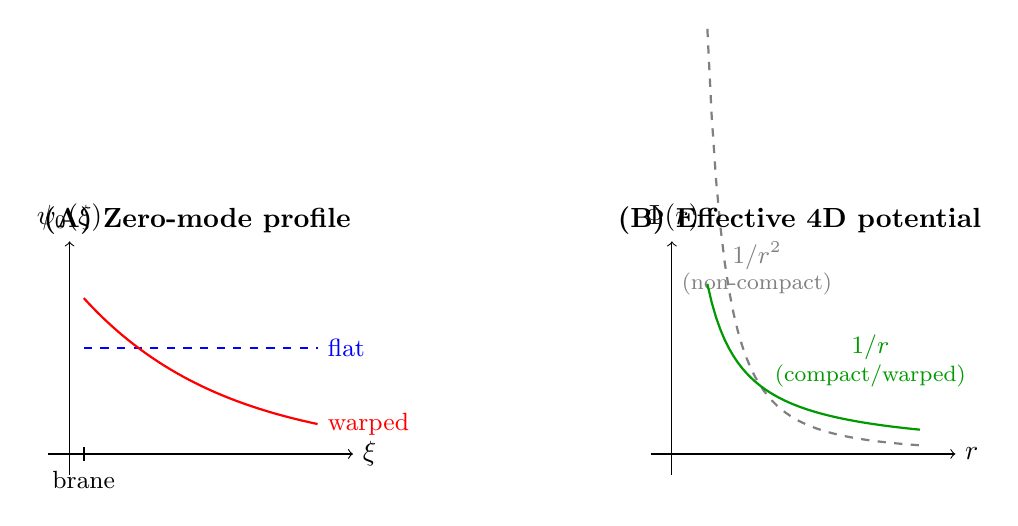
\begin{tikzpicture}[scale=0.9]
% Panel A: Mode profile
\begin{scope}[shift={(-4.5,0)}]
    \draw[->] (-0.3,0) -- (4,0) node[right] {$\xi$};
    \draw[->] (0,-0.3) -- (0,3) node[above] {$\psi_0(\xi)$};

    % Flat mode (dashed)
    \draw[dashed, blue, thick] (0.2,1.5) -- (3.5,1.5) node[right, font=\small] {flat};

    % Warped mode (solid)
    \draw[red, thick, domain=0.2:3.5, samples=50]
        plot (\x, {2.2*exp(-0.5*(\x-0.2))}) node[right, font=\small] {warped};

    % Brane marker
    \draw[thick] (0.2,-0.1) -- (0.2,0.1);
    \node[below, font=\small] at (0.2,-0.1) {brane};

    \node[font=\bfseries] at (1.8,3.3) {(A) Zero-mode profile};
\end{scope}

% Panel B: Potential scaling
\begin{scope}[shift={(4,0)}]
    \draw[->] (-0.3,0) -- (4,0) node[right] {$r$};
    \draw[->] (0,-0.3) -- (0,3) node[above] {$\Phi(r)$};

    % 1/r^2 (non-compact)
    \draw[dashed, gray, thick, domain=0.5:3.5, samples=50]
        plot (\x, {1.5/(\x*\x)});
    \node[gray, font=\small] at (1.2,2.8) {$1/r^2$};
    \node[gray, font=\footnotesize] at (1.2,2.4) {(non-compact)};

    % 1/r (compact/warped)
    \draw[green!60!black, thick, domain=0.5:3.5, samples=50]
        plot (\x, {1.2/\x});
    \node[green!60!black, font=\small] at (2.8,1.5) {$1/r$};
    \node[green!60!black, font=\footnotesize] at (2.8,1.1) {(compact/warped)};

    \node[font=\bfseries] at (1.8,3.3) {(B) Effective 4D potential};
\end{scope}
\end{tikzpicture}
\caption{%
\textbf{(A)}~Zero-mode profile $\psi_0(\xi)$: constant for flat compactification,
localized near brane for warped geometry.
\textbf{(B)}~Effective 4D gravitational potential: non-compact gives $1/r^2$
(excluded by observation), compact/warped recovers $1/r$ (Newtonian).
\emph{Schematic only, not to scale.}
}
\label{fig:schematic}
\end{figure}

%==============================================================================
\section{Epistemic Classification Table}
\label{sec:epistemic}

\begin{table}[h]
\centering
\caption{Epistemic ledger for derivation v13}
\label{tab:epistemic}
\begin{tabular}{@{}lcc@{}}
\toprule
\textbf{Element} & \textbf{Tag} & \textbf{Source/Status} \\
\midrule
5D EH action structure & [I] & Imported from GR/RS literature \\
GHY boundary term & [I] & York (1972), Gibbons--Hawking (1977) \\
Brane tension term & [P] & Standard RS ansatz \\
Linearization ansatz & [M] & Mathematical expansion \\
5D Green's function $\sim 1/r^2$ & [D] & Derived from 5D Laplacian \\
Non-compact $\Rightarrow$ excluded & [BL] & Observation: $\Phi \propto 1/r$ \\
KK decomposition & [I] & Kaluza (1921), Klein (1926) \\
Eigenvalue equation for $\psi_n$ & [D] & Derived from variation \\
Normalization condition & [M] & Definition of unit norm \\
Zero-mode $\Rightarrow$ $1/r$ & [D] & Derived from 4D effective theory \\
$\Mpl^2 = \Mfive^3 \calI$ & [D] & Derived (dimensional reduction) \\
$\GN = 1/(8\pi\Mpl^2)$ & [M] & Definition \\
Flat case: $\calI = L$ & [D] & Derived (explicit integration) \\
RS case: $\calI = 2L$ or $1/k$ & [I] & RS model (1999) \\
Warp factor $A(\xi)$ & [P/I] & Must be specified by EDC \\
$\Mfive$ value & [P/Cal] & Postulate or calibration \\
\bottomrule
\end{tabular}
\end{table}

\noindent
\textbf{Legend:}
[M]~Mathematical identity;
[D]~Derived within this note;
[Dc]~Derived conditional on stated assumption;
[P]~Postulate;
[I]~Imported from literature;
[BL]~Baseline (observational input);
[Cal]~Calibrated to observation.

%==============================================================================
\section{Conclusion}
\label{sec:conclusion}

\subsection{What v13 Closes}

\begin{enumerate}
    \item \textbf{Functional form:} The relationship $\GN = 1/(8\pi\Mfive^3\calI)$
          is now explicit.

    \item \textbf{Normalization slot:} The integral $\calI = \int d\xi \, e^{4A} |\psi_0|^2$
          is identified as the key quantity linking 5D and 4D.

    \item \textbf{Exclusion:} Non-compact extra dimensions are excluded by
          observation ($1/r^2$ vs $1/r$).

    \item \textbf{Recovery mechanism:} Compact or warped geometries restore
          4D gravity via a normalizable zero-mode.
\end{enumerate}

\subsection{What Remains Open}

For EDC to close BLOCK-003, it must provide:
\begin{center}
\begin{tabular}{@{}lll@{}}
\toprule
\textbf{Gap} & \textbf{Required Input} & \textbf{Status} \\
\midrule
Warp factor & $A(\xi)$ from EDC dynamics & OPEN \\
Compactification scale & $L$ or equivalent & OPEN \\
5D Planck mass & $\Mfive$ from first principles & OPEN \\
One calibration & $\GN^{\text{obs}}$ or $\ell_P^{\text{obs}}$ & Available [BL] \\
\bottomrule
\end{tabular}
\end{center}

\subsection{One-Line Outcome}

\begin{center}
\fbox{\parbox{0.9\textwidth}{\centering
\textbf{BRIDGE SLOT FOUND:} $\GN$ reduces to $\Mfive^3 \calI$; \\
EDC must compute $\calI$ or provide one calibration scale.
}}
\end{center}

%==============================================================================
\section*{References}

\begin{enumerate}
    \item L.~Randall and R.~Sundrum, ``A Large Mass Hierarchy from a Small Extra
          Dimension,'' Phys.\ Rev.\ Lett.\ \textbf{83}, 3370 (1999).
    \item L.~Randall and R.~Sundrum, ``An Alternative to Compactification,''
          Phys.\ Rev.\ Lett.\ \textbf{83}, 4690 (1999).
    \item G.~W.~Gibbons and S.~W.~Hawking, ``Action Integrals and Partition
          Functions in Quantum Gravity,'' Phys.\ Rev.\ D \textbf{15}, 2752 (1977).
    \item J.~W.~York, ``Role of Conformal Three-Geometry in the Dynamics of
          Gravitation,'' Phys.\ Rev.\ Lett.\ \textbf{28}, 1082 (1972).
    \item R.~Maartens, ``Brane-World Gravity,'' Living Rev.\ Relativ.\ \textbf{7},
          7 (2004).
\end{enumerate}

\end{document}
